\subsection{Action Frames Generation}
This subsection evaluates our ability to automatically infer action 
frames of verbs. 
clusters the verbs by their argument concepts and then 
compares our result with FrameNet.

First we prepare two types of context for each verb as follows:
\begin{description}\setlength{\itemsep}{-\itemsep}
\item [Subjects only] Get the top 20 subject concepts of a verb, and pick the subject only instances from corpus by IsA relation to generate subject concepts.
\item [Objects only] Get the top 20 object concepts of a verb, and pick the object only instances from corpus by IsA relation to generate object concepts.
\end{description}
Then we combine \textbf{Subjects only} and \textbf{Objects only} to generate the feature vector of a verb, as the input for clustering.
After generating the features for every verbs, we get the clusters of verbs via a Fuzzy C-means
clustering \cite{dunn73:fuzzycmeans}.
The above process returns for every verbs the coefficients
of being in each cluster, namely $Co(v,c)$. In order to find the 
strongest signal of a verb belonging to a cluster, we design 
the following condition to determine if a verb $v_i$ cluster 
belongs to $c_j$:
$$
Co(v_i,c_j) \geq \mu_{v_i} + 3 \times \sigma_{v_i}
$$
Where $\mu_{v_i}$ and $\sigma_{v_i}$ represents the average and 
standard deviation of the coefficients of being in clusters set 
of verb $v_i$. In the case that a verb can't find any strong signal of 
belonging to a cluster, it is a cluster on its own.

To evaluate the accuracy of the inferred clusters or action frames, 
we compute the Jaccard Similarity between each cluster and frames in 
the FrameNet. If that similarity with frame $f$ is larger than 
than $\alpha$, the cluster is considered to have found a corresponding
frame in FrameNet. 
In this process, we only consider the clusters and FrameNet frames 
with more than one verb, because we can only determine (or
disambiguate) the sense of a frame if it contains more than one member. 
In our experiment, we get clusters from $200$ verbs, 
and set $\alpha$ to be $0.25$. \figref{fig:cluster} shows that we 
can get the best result with the number of clusters preset to $130$. 
Our final result shows that our Action frames can be similar 
to 41\% percentage of FrameNet frames. A selected number of
our action frames are shown in \tabref{cluster}.
\begin{table*}[th]
\small
\centering
%\scriptsize
\caption{Automatic Generation of Action Frames}
\begin{tabular}{|l|l|l|c|}
\hline
AC frames & FrameNet frames & Verbs in FrameNet& Similarity \\
\hline \hline
offer	produce	save	avoid & Offering & offer serve & 0.20 \\
\hline
need	purchase & Needing & need require & 0.33 \\
\hline
describe explain & Statement & allow describe maintain & 0.25 \\
\hline
win	fall& Finish\_game & lose win & 0.33 \\
\hline
write	share	tell & Spelling\_and\_pronouncing & say write &0.25 \\
\hline
call	ask & Request & ask call tell &0.67 \\
\hline
develop	improve	test & Cause\_to\_make\_progress & develop improve & 0.67 \\
\hline
come stay & Residence & live stay & 0.33 \\
\hline
\end{tabular}
\label{cluster}
\end{table*}

\begin{figure}[th]
\centering
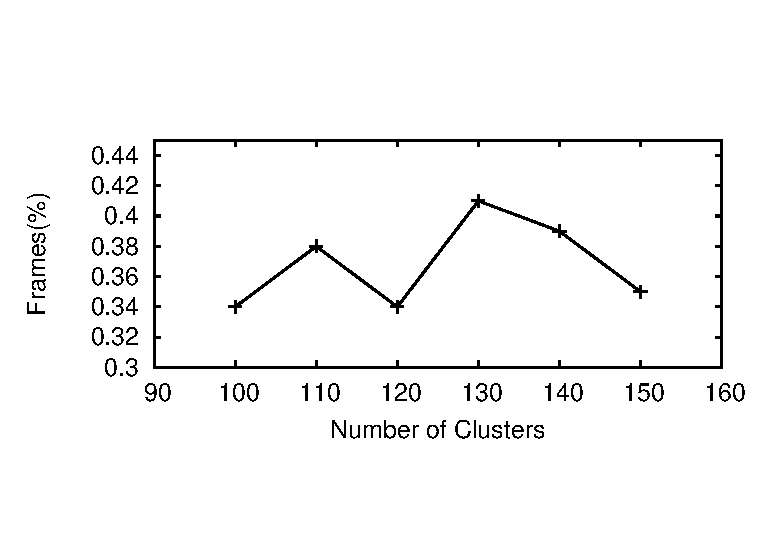
\epsfig{file=figure/cluster.eps,width=.8\columnwidth}
\vspace*{-4ex}
\caption{Numbers of Clusters vs. Number of Matching Frames in FrameNet}
\label{fig:cluster}
\end{figure}


